\input{../header.tex}
\usepackage{menukeys}
\usepackage{fontawesome6}
\usepackage{graphicx}
\usepackage{breakurl}

\usepackage{subcaption}

\begin{document}

% Change the following values to true to show the solutions or/and the hints
\ShowSolutiontrue
\ShowConseiltrue
\ShowWarningtrue
\ShowNotetrue

\titre
\cours{Prise en main de l'environnement de travail}

Le but de cette séance est d'installer et de configurer les outils sur \textbf{Windows} qui seront utilisés tout au long du semestre. 

\subsection*{Prérequis}
Avant d'installer les outils de développement, vous devez vous assurer d'avoir installé Python et le kit de développement Java (Java).
\begin{enumerate}
    \item \textbf{Python}. Pour installer Python, rendez-vous sur le site officiel de Python \url{https://www.python.org/downloads}. Sélectionnez la dernière version de Python et cliquez sur \textbf{Download Python 3.13.7} comme dans la capture d'écran ci-dessous.
    \begin{figure}[h!]
        \centering
        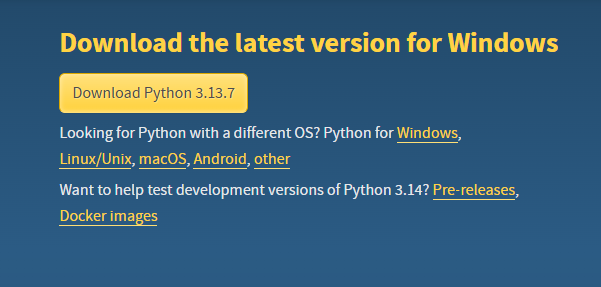
\includegraphics[width=0.7\textwidth]{img/win/download-python.png}
    \end{figure}

    \begin{attention}
        Une fois le fichier exécutable téléchargé, cliquez sur \texttt{Add python.exe to PATH} comme dans l'image ci-dessous. 
    \end{attention}
    
    
    \begin{figure}[h!]
        \centering
        \fbox{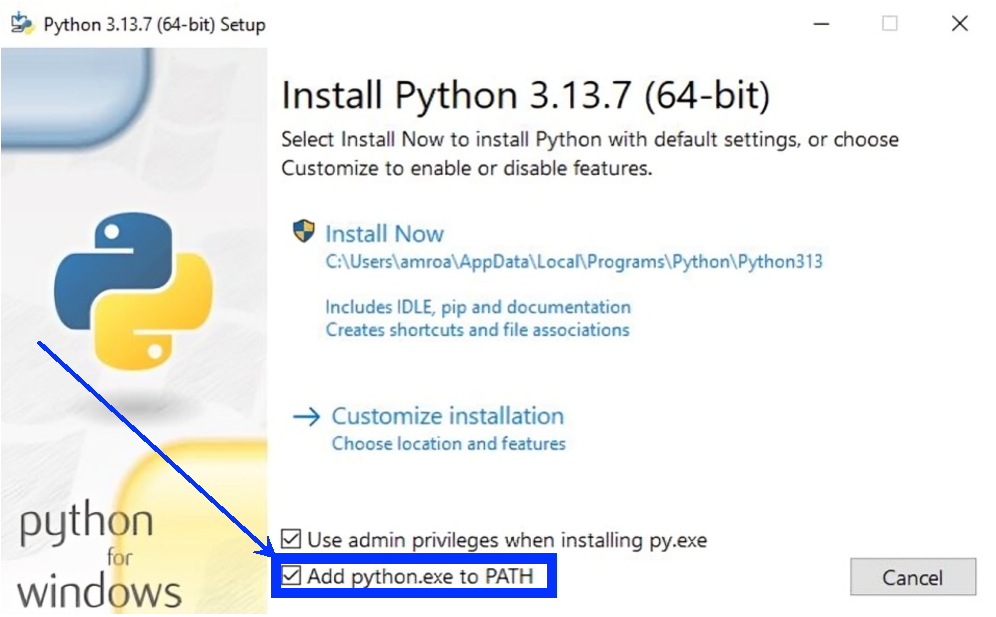
\includegraphics[width=0.7\textwidth]{img/win/python-install.pdf}}
    \end{figure}
    Pour tester que tout fonctionne, ouvrez votre terminal (command prompt ou powershell) et tapez la commande \lstinline{python --version}, vous devriez avoir la fenêtre ci-dessous.

    \begin{figure}[h!]
        \centering
        \fbox{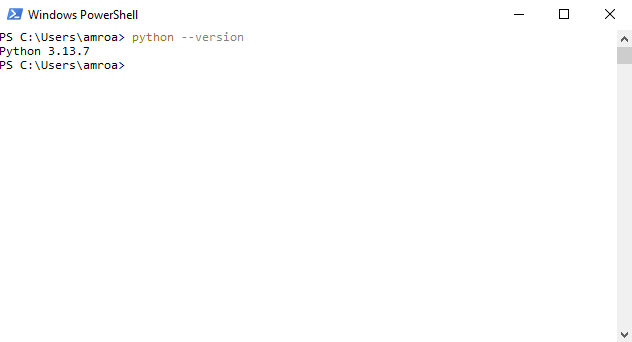
\includegraphics[width=0.5\textwidth]{img/win/python-verify.png}}
        \caption{Aperçu du powershell à la fin de l'installation de Python}
    \end{figure}

    \newpage

    \item \textbf{Java Development Kit (JDK)}. Le JDK contient tout 
    le nécessaire pour développer des applications Java. 
    Pour le télécharger, se rendre sur le site 
    d'Oracle \url{https://www.oracle.com/java/technologies/downloads/} 
    et sélectionner la version correspondante 
    à Windows: \texttt{x64 Installer}. \newline 
    
    Vous verrez ensuite une fenêtre avec le texte \textbf{Voulez-vous autoriser cette application à apporter des modifications à votre appareil?} Cliquez oui. Gardez les options sélectionnées par défaut. Après installation, vous devriez voir \texttt{javac 25} en exécutant la commande \texttt{javac --version} dans powershell ou command prompt. 
\end{enumerate}

\subsection*{IntelliJ}

L'IDE (Integrated Development Environment) qui sera utilisé tout au long du semestre sera la version gratuite de \textbf{IntelliJ}, Community Edition. Pour l'utiliser, vous devez suivre les étapes suivantes:
\begin{enumerate}
    \item Télécharger la version community d'IntelliJ directement sur le site internet \url{https://www.jetbrains.com/edu-products/download/?section=idea}. Dès que vous cliquez, vous verrez une fenêtre avec le texte \textbf{Voulez-vous autoriser cette application à apporter des modifications à votre appareil?} Cliquez oui. 
    \begin{attention}
    Il ne faut pas importer les settings que vous avez dans un autre editeur de code (par exemple, Visual Studio Code) dans IntelliJ.
    \end{attention}
    Cliquez sur \texttt{\faPlus New Project} dans la fenêtre d'accueil ci-dessous.
    \begin{figure}[h!]
        \centering
        \fbox{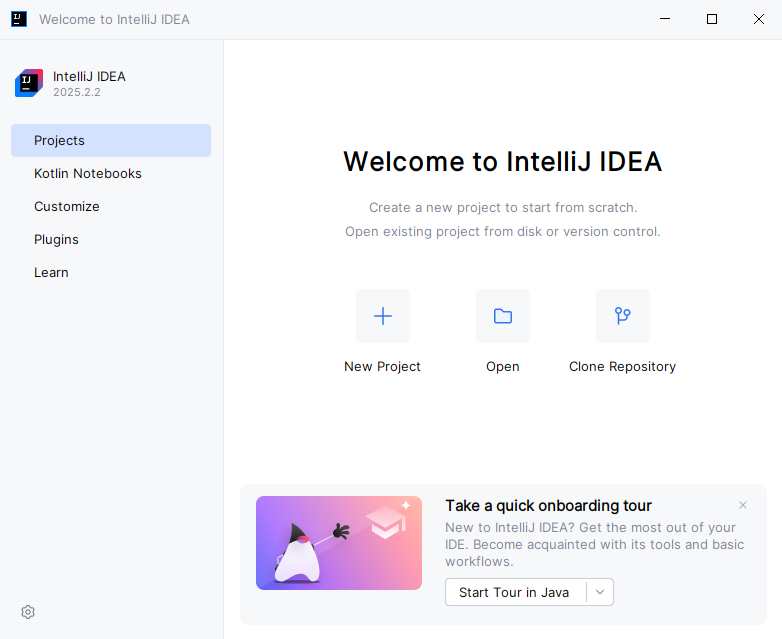
\includegraphics[width=0.4\textwidth]{img/win/intellij-welcome.PNG}}
    \end{figure}
    \item Pour utiliser Python sur IntelliJ, 
    vous devez installer le plugin 
    Python en cliquant sur \texttt{More via plugins...} 
    et ensuite \texttt{OK}.

    \begin{figure}[h!]
    \centering
    \begin{subfigure}[t]{0.45\textwidth}
        \centering
        \fbox{
\includegraphics[width=\textwidth]{img/win/pythonplugin1.pdf}}
        \caption{Création d'un nouveau projet - Install Plugin}
        \label{fig:sub1}
    \end{subfigure}
    \hfill
    \begin{subfigure}[t]{0.45\textwidth}
        \centering
        \raisebox{0.7cm}{ % adjust the value as needed
            \fbox{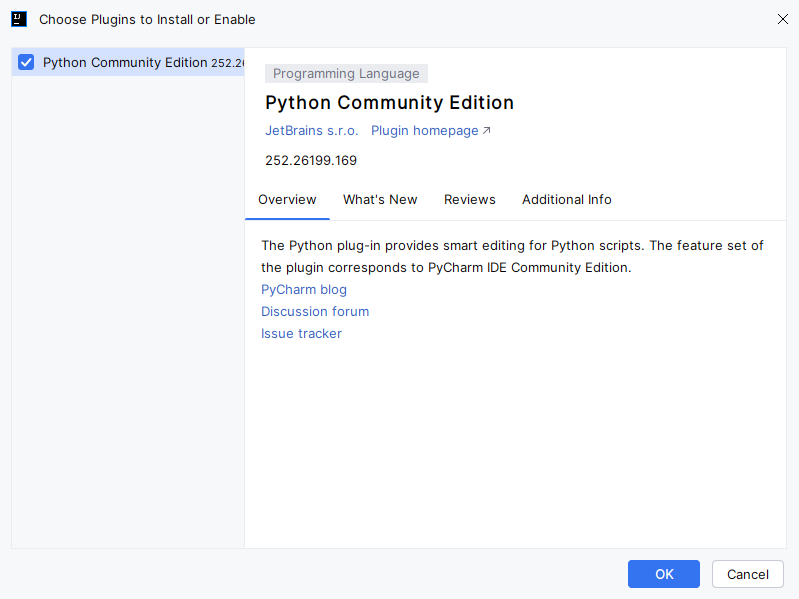
\includegraphics[width=\textwidth]{img/win/pythonplugin2.PNG}}
        }
        \caption{Installation du plugin Python}
        \label{fig:sub2}
    \end{subfigure}
    \caption{Utilisation de Python dans Intellij}
    \label{fig:installpython}
\end{figure}
    
    \item Pour créer un nouveau projet, cliquez sur \texttt{Create} à partir de la fenêtre d'accueil, sélectionnez Python ou Java sur le menu latéral à gauche. Définissez l'emplacement de votre kit de développement logiciel et donnez un nom à votre projet (Assurez-vous de choisir une version Python $>=$ 3.11). Cliquez sur \texttt{Create}.
    \begin{figure}[ht]
    \centering
    \begin{subfigure}[t]{0.45\textwidth}
        \centering
        \fbox{
\includegraphics[width=\textwidth]{img/win/javaproject.png}}
        \caption{Création d'un projet Java}
        \label{fig:sub1}
    \end{subfigure}
    \hfill
    \begin{subfigure}[t]{0.45\textwidth}
        \centering
        \raisebox{0.0cm}{ % adjust the value as needed
            \fbox{
\includegraphics[width=\textwidth]{img/win/pythonproject.png}}
        }
        \caption{Création d'un projet Python}
        \label{fig:sub2}
    \end{subfigure}
    \label{fig:createproject}
\end{figure}
\end{enumerate}


\subsection*{Votre premier programme}

\begin{itemize}
    \item \textbf{Python: }\url{https://www.jetbrains.com/help/idea/creating-empty-python-project.html}
    \item \textbf{Java: }\burl{https://www.jetbrains.com/help/idea/creating-and-running-your-first-java-application.html#run_app}
\end{itemize}
\newpage
\subsection*{Résolution Bug Windows}
Sur Windows, lorsque vous tentez d'exécuter un fichier java, il se peut que le message d'erreur suivant s'affiche :\\
 
\begin{Example}{\faTriangleExclamation \quad Message d'erreur}
    \textbf{`javac' n'est pas reconnue comme une commande interne ou externe.}
\end{Example}
 
Dans ce cas, suivez les étapes suivantes :
 
\begin{enumerate}
    \item Ouvrez votre panneau de configuration $>$ Système et sécurité $>$ Système $>$ Paramètres systèmes avancés. La fenêtre suivante devrait s'afficher.\\
    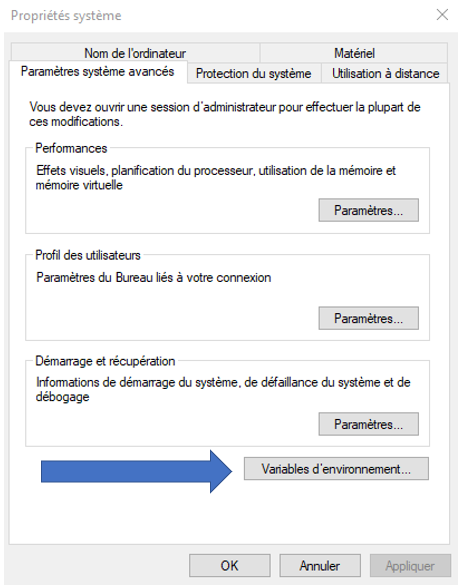
\includegraphics[height = 10cm]{img/Res1.PNG}
    \\
    \item Sélectionnez Variables d'environnement. Dans variables système, identifiez la variable "Path", sélectionnez là et choisissez modifier.\\
    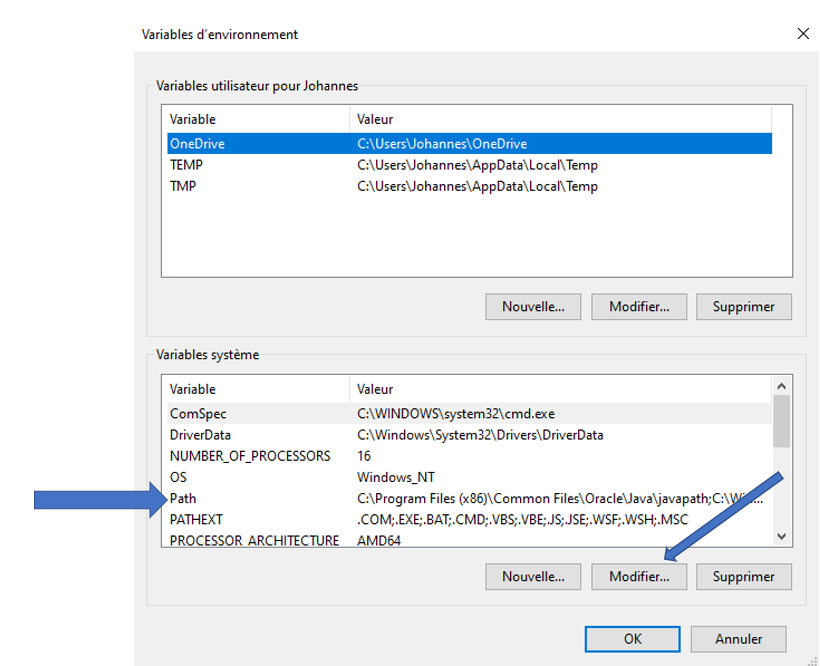
\includegraphics[width=16cm]{img/Res2.PNG}
    \item Ouvrez votre explorateur de fichiers et trouvez le chemin d'accès à \textbf{javac} et \textbf{java}. \\Par exemple : $C:\backslash Program Files\backslash Common Files\backslash Oracle\backslash Java \backslash javapath.$\\
    \item Copiez ce chemin d'accès et copiez-le à la première ligne de la variable d'environnement Path.\\\
    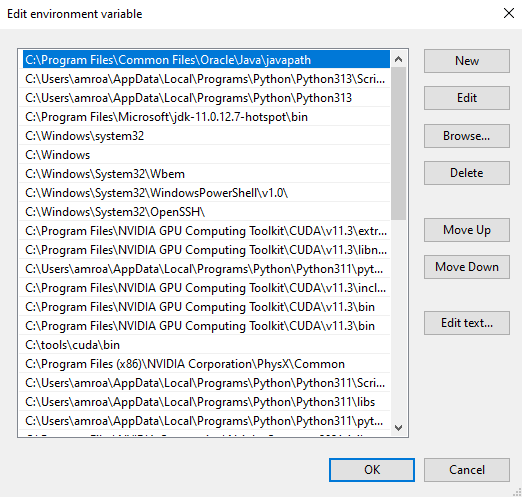
\includegraphics[width=15cm]{img/win/environment-variables.PNG}\\
    \item Faites OK. Puis redémarrez votre ordinateur.
    \item Ouvrez votre Terminal, Naviguez vers votre fichier .java et tapez :
        \begin{enumerate}
            \item \lstinline{javac VotreProgramme.java} (Cette commande va créer un fichier avec une extension \lstinline{.class})
            \item \lstinline{java VotreProgramme} (Cette commande va exécuter votre programme. À noter que votre programme doit être le fichier qui contient la classe \lstinline{main}).
        \end{enumerate}
    
\end{enumerate}


\end{document}
